\documentclass[border={2pt -1cm 2pt -1cm},convert={density=150,outext=.png}]{standalone}
\usepackage{mathpazo}
\usepackage{tikz}
\usetikzlibrary{arrows,decorations.pathmorphing,backgrounds,positioning,fit,shapes.misc,calc}
%
\tikzset{
pipestage/.style={
    rounded rectangle,
    minimum width=20mm,
    inner sep=2pt,
    draw=black,
    node distance=15mm,
    font=\ttfamily
},
pipestageinner/.style={
    pipestage,
    minimum width=10mm,
    node distance=3mm,
    font=\ttfamily\small
},
pipedep/.style={
    red,semithick,>=stealth'
},
pipedep2/.style={
    red,very thick,>=stealth'
},
pipepixdep/.style={
    red,thick,densely dotted
},
barrier/.style={
    rectangle,
    minimum width=40mm,
    minimum height=8mm,
    inner sep=2pt,
    draw=black,
    font=\ttfamily
},
barrierport/.style={
    rectangle,
    minimum width=40mm,
    draw=black,
    inner sep=2pt,
    font=\ttfamily\footnotesize
},
}
%
\tikzset{pipeline/.pic={
%
\node [pipestageinner] (vs) {VERT};
\node [pipestageinner,right=of vs] (fs) {FRAG};
\node [pipestageinner,right=of fs] (ca) {COLR};
\node [pipestageinner,right=of ca] (comp) {COMP};
\node [pipestageinner,right=of comp] (xfer) {XFER};
%
\node [pipestage,above=of ca] (top) {TOP};
\node [pipestage,below=of ca] (bottom) {BOTTOM};
%
\draw [->,pipepixdep] (vs) -- (fs);
\draw [->,pipepixdep] (fs) -- (ca);
\draw (top.south)
    edge [->,pipedep,in=90,out=270] (vs)
    edge [->,pipedep,in=90,out=270] (fs)
    edge [->,pipedep,in=90,out=270] (ca)
    edge [->,pipedep,in=90,out=270] (comp)
    edge [->,pipedep,in=90,out=270] (xfer);
\draw (bottom.north)
    edge [<-,pipedep,in=270,out=90] (vs)
    edge [<-,pipedep,in=270,out=90] (fs)
    edge [<-,pipedep,in=270,out=90] (ca)
    edge [<-,pipedep,in=270,out=90] (comp)
    edge [<-,pipedep,in=270,out=90] (xfer);
%
\begin{scope}[on background layer]
\node (bg) [draw,fit=(top) (bottom) (vs) (xfer)] {};
\node [anchor=north west] at (bg.north west) {#1};
\end{scope}
%
}}
%
\tikzset{pics/barrier/.style 2 args={code={
%
\node (box) [barrier] {PipelineBarrier};
\node (in) [barrierport,anchor=south] at (box.north) {#1};
\node (out) [barrierport,anchor=north] at (box.south) {#2};
%
}}}


\begin{document}
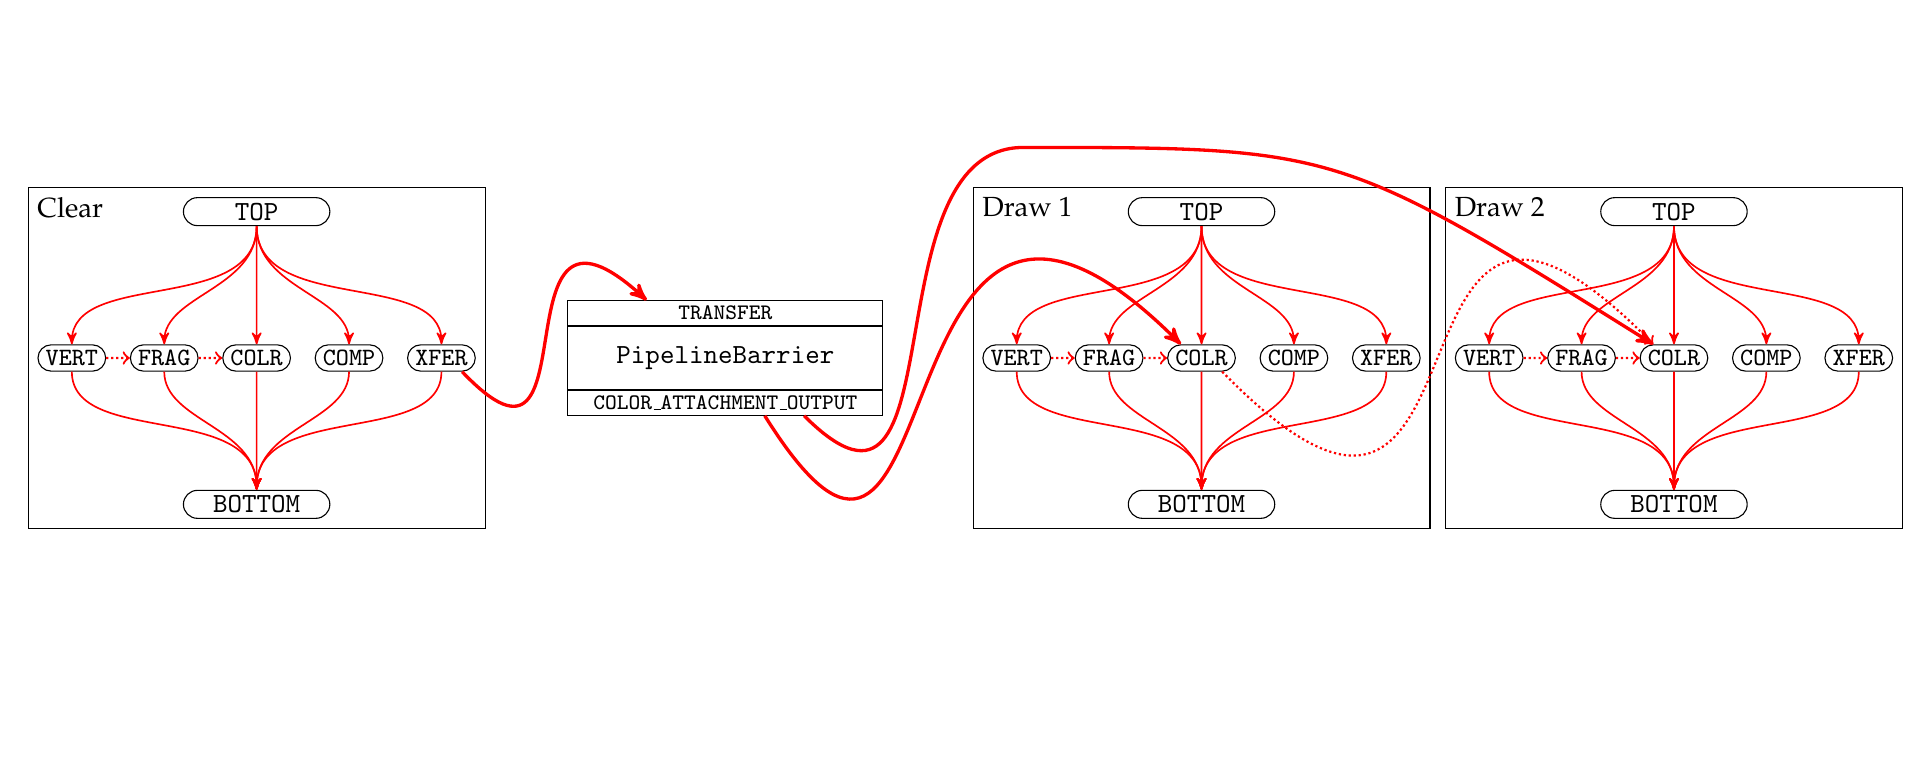
\begin{tikzpicture}

\pic[] (clear-) {pipeline=Clear};
\pic[xshift=12cm] (draw1-) {pipeline=Draw 1};
\pic[xshift=18cm] (draw2-) {pipeline=Draw 2};

%\draw [->,pipepixdep] (clear-ca.south east) .. controls ($ (clear-ca) + (4cm,-4cm) $) and ($ (draw1-ca) - (4cm,-4cm) $) .. (draw1-ca.north west);
\draw [->,pipepixdep] (draw1-ca.south east) .. controls ($ (draw1-ca) + (4cm,-4cm) $) and ($ (draw2-ca) - (4cm,-4cm) $) .. (draw2-ca.north west);

\pic[xshift=8.3cm] (barrier1-) {barrier={TRANSFER}{COLOR\_ATTACHMENT\_OUTPUT}};

\draw [->,pipedep2] (clear-xfer.south east) .. controls ($ (clear-xfer) + (2cm,-2cm) $) and ($ (barrier1-in) - (3cm,-2cm) $) .. ($ (barrier1-in.north) - (1cm,0) $);
\draw [->,pipedep2] ($ (barrier1-out.south) + (0.5cm,0) $) .. controls ($ (barrier1-out.south) + (3cm,-4cm) $) and ($ (draw1-ca.north west) - (4cm,-4cm) $) .. (draw1-ca.north west);
\draw [->,pipedep2] ($ (barrier1-out.south) + (1cm,0) $) .. controls ($ (barrier1-out.south) + (3cm,-2cm) $) and ($ (draw1-ca.north west) - (4cm,-2.5cm) $) .. ($ (draw2-ca.north west) - (8cm,-2.5cm) $) .. controls ($ (draw2-ca.north west) - (4cm,-2.5cm) $) .. (draw2-ca.north west);

\end{tikzpicture}
\end{document}
